\documentclass{article}
\usepackage{tikz}

\pagestyle{empty}


\setlength{\parskip}{.5cm}
\setlength{\parindent}{0cm}
\setlength{\topmargin}{0cm}
\setlength{\voffset}{-2cm}
\setlength{\hoffset}{-3.5cm}
\setlength{\textwidth}{19cm}
\setlength{\textheight}{25cm}
\thispagestyle{empty}
\pagestyle{empty}

\newcommand{\point}[2]{\filldraw[black] (\xoffset+7+#1*0.5,\yoffset+12+#2*0.5) circle (2pt);}
\newcommand{\linepoints}[4]{%
  \point{#1}{#2}%
  \point{#3}{#4}%
  \draw(\xoffset+7+#1*0.5,\yoffset+12+#2*0.5) -- (\xoffset+7+#3*0.5,\yoffset+12+#4*0.5);%
  }

\begin{document}
\begin{center}
  \begin{tikzpicture}
    \foreach \xoffset / \yoffset in { 0 / -1 } {
      \draw[step=.5cm,teal!30](0,0)grid(18.5,18.5);
      \draw[->](\xoffset+7,\yoffset+6.5) -> (\xoffset+7,\yoffset+18);
      \draw[->](\xoffset+0.5,\yoffset+12) -- (\xoffset+15,\yoffset+12);
      \foreach \x in {1,2,3,4,5,6,7,8,9,10,11,12,13,14} {
        \draw(\xoffset+\x,\yoffset+11.9) -- (\xoffset+\x,\yoffset+12.1);
        \draw(\xoffset+\x+0.5,\yoffset+11.9) -- (\xoffset+\x+0.5,\yoffset+12.1);
      }

      \foreach \x in { -5, -10, 5, 10 } {
        \draw(\xoffset+6.95+\x/2, \yoffset + 11.9) node[anchor=north] {\large \x};
      }
      
      \foreach \y in { -5, -10, 5, 10 } {
        \draw(\xoffset+6.6, \yoffset + 12.25 + \y/2) node[anchor=north] {\large \y};
      }
      
      \foreach \y in {7,8,9,10,11,12,13,14,15,16,17} {
        \draw(\xoffset+6.9,\yoffset+\y) -- (\xoffset+7.1,\yoffset+\y);
        \draw(\xoffset+6.9,\yoffset+\y+0.5) -- (\xoffset+7.1,\yoffset+\y+0.5);
      }
      \linepoints{-2}{2}{3}{0}
      \linepoints{3}{0}{4}{2}
    }
               
    
  \end{tikzpicture}
\end{center}

\end{document}

